\documentclass[tikz,border=3pt]{standalone}
\usepackage[T1]{fontenc}
\usepackage{amsmath}
\usetikzlibrary{arrows.meta,positioning,fit,backgrounds,calc}

\definecolor{ink}{HTML}{24313A}
\definecolor{blue}{HTML}{DCEAF7}
\definecolor{blueedge}{HTML}{3E7896}
\definecolor{amber}{HTML}{F8E7C8}
\definecolor{amberedge}{HTML}{B87818}
\definecolor{teal}{HTML}{D9EEE9}
\definecolor{tealedge}{HTML}{167A69}
\definecolor{grayfill}{HTML}{F1F3F4}
\definecolor{grayedge}{HTML}{7C878E}
\definecolor{muted}{HTML}{65737C}

\begin{document}
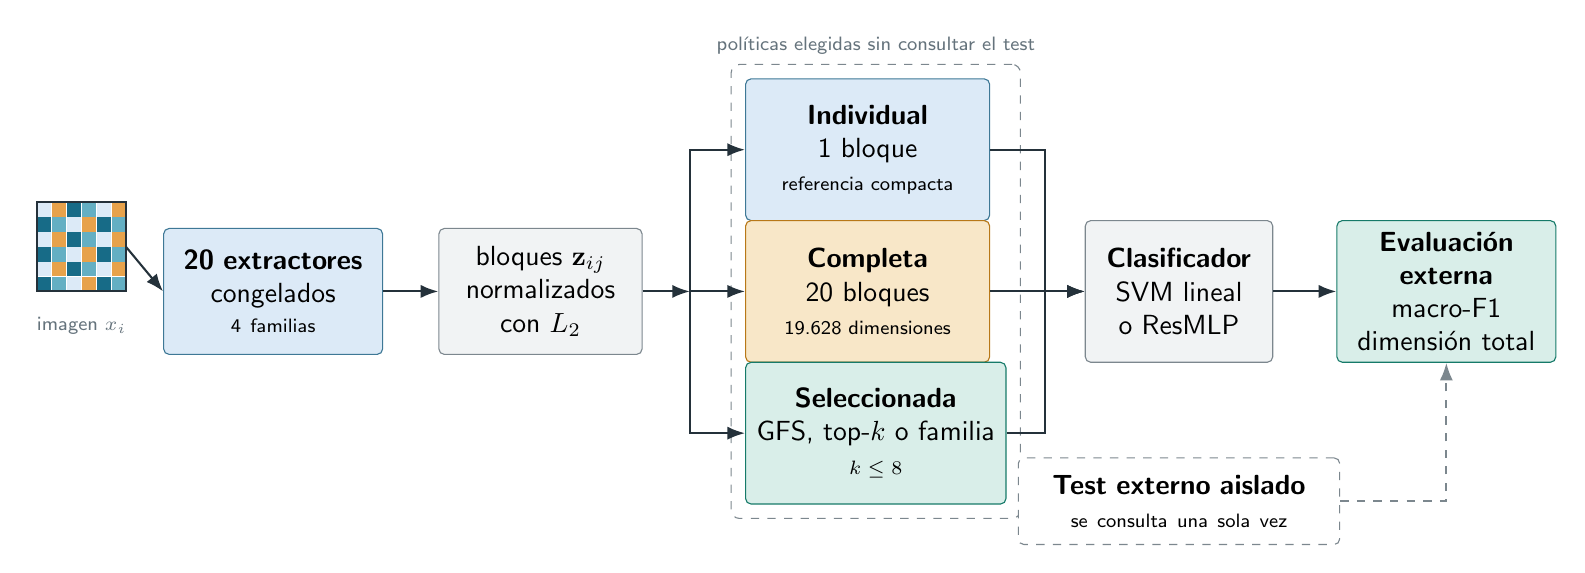
\begin{tikzpicture}[
  font=\sffamily,
  >=Latex,
  flow/.style={->, draw=ink, line width=.75pt},
  box/.style={rounded corners=2pt, draw=grayedge, fill=grayfill,
              minimum height=10mm, align=center, inner sep=4pt},
  policy/.style={rounded corners=2pt, minimum width=31mm,
                 minimum height=18mm, align=center, inner sep=4pt},
  note/.style={font=\sffamily\scriptsize, text=muted, align=center},
  title/.style={font=\sffamily\small\bfseries, text=ink}
]

% Entrada con textura esquemática.
\coordinate (imgbase) at (0,0);
\foreach \r in {0,...,5}{
  \foreach \c in {0,...,5}{
    \pgfmathtruncatemacro{\shadeidx}{mod(2*\r+\c,4)}
    \ifcase\shadeidx
      \definecolor{tile}{HTML}{176B87}
    \or
      \definecolor{tile}{HTML}{64AFC3}
    \or
      \definecolor{tile}{HTML}{DCEAF7}
    \or
      \definecolor{tile}{HTML}{E7A24B}
    \fi
    \fill[tile] ($(imgbase)+(0.19*\c,0.19*\r)$) rectangle ++(0.18,0.18);
  }
}
\draw[ink,line width=.7pt] (imgbase) rectangle ++(1.13,1.13);
\node[note, below=2mm] at ($(imgbase)+(0.565,0)$) {imagen $x_i$};

\node[box, fill=blue, draw=blueedge, right=16mm of imgbase, anchor=west,
      text width=25mm, minimum height=16mm] (extract) {\textbf{20 extractores}\\congelados\\[-1pt]\scriptsize 4 familias};
\node[box, right=7mm of extract, text width=23mm, minimum height=16mm] (norm)
      {bloques $\mathbf z_{ij}$\\normalizados con $L_2$};
\draw[flow] ($(imgbase)+(1.13,.565)$) -- (extract.west);
\draw[flow] (extract) -- (norm);

\node[policy, fill=blue, draw=blueedge, right=13mm of norm, yshift=18mm] (individual)
      {\textbf{Individual}\\1 bloque\\\scriptsize referencia compacta};
\node[policy, fill=amber, draw=amberedge, right=13mm of norm] (complete)
      {\textbf{Completa}\\20 bloques\\\scriptsize 19.628 dimensiones};
\node[policy, fill=teal, draw=tealedge, right=13mm of norm, yshift=-18mm] (selected)
      {\textbf{Seleccionada}\\GFS, top-$k$ o familia\\\scriptsize $k\leq 8$};

\coordinate (fork) at ($(norm.east)+(6mm,0)$);
\draw[flow] (norm.east) -- (fork);
\draw[flow] (fork) |- (individual.west);
\draw[flow] (fork) -- (complete.west);
\draw[flow] (fork) |- (selected.west);

\node[box, fill=grayfill, right=12mm of complete, text width=21mm,
      minimum height=18mm] (clf) {\textbf{Clasificador}\\SVM lineal\\o ResMLP};
\draw[flow] (individual.east) -| ($(clf.west)+(-5mm,0)$) -- (clf.west);
\draw[flow] (complete.east) -- (clf.west);
\draw[flow] (selected.east) -| ($(clf.west)+(-5mm,0)$) -- (clf.west);

\node[box, fill=teal, draw=tealedge, right=8mm of clf, text width=25mm,
      minimum height=18mm] (measure) {\textbf{Evaluación externa}\\macro-F1\\dimensión total};
\draw[flow] (clf) -- (measure);

\begin{scope}[on background layer]
  \node[rounded corners=3pt, draw=grayedge, dashed, inner sep=5pt,
        fit=(individual)(complete)(selected), label={[note]above:políticas elegidas sin consultar el test}] {};
\end{scope}

\node[box, fill=white, draw=grayedge, dashed, below=12mm of clf,
      text width=38mm, minimum height=11mm] (test)
      {\textbf{Test externo aislado}\\\scriptsize se consulta una sola vez};
\draw[flow, dashed, draw=grayedge] (test.east) -| (measure.south);

\end{tikzpicture}
\end{document}
